\chapter{Causal Models}
\section{The do-operator and Interventional Distributions}
As you have undoubtedly heard many times in statistics classes, “correlation is
not causation.” A mere association between two variables does not necessarily
mean that one of those variables causes the other. For this reason, the
\textbf{randomized controlled experiment} is considered the standard of statistics.

We can define a randomized controlled experiment as an experiment in which all
the \textbf{factors} that influence the outcome of the experiment are either
static or vary at random, except for one. This implies that any change in the
outcome variable must be due to that one input variable, so we can control a factor
and study how the outcome changes. This type of experiment allows us to find causal
relationships, so we can answer causal queries.

In cases where randomized controlled experiments are not practical, researchers
instead perform \textbf{observational studies}, in which they merely record data,
rather than control it. In these cases, the problem is that is difficult to
untangle the effects of different variables.

We can summarize the difference between these two types of studies, with reference
to the Figure~\ref{fig:causal}, as follows:
\begin{itemize}
      \item \textbf{Intervening}: we change the system assigning values to the a
            variable and observing the effect on the other variables. When we
            intervene to fix the value of a variable, we curtail the natural
            tendency of that variable to vary in response to other variables in
            nature. This amounts to performing surgery on the graphical model,
            which we do by removing all edges directed into that variable.
            Intervening would be to take the whole population and give everyone
            treatment. This is possible if we can control the experiment because
            we can apply a treatment to the entire population.
      \item \textbf{Conditioning}: we merely narrow our focus to the subset of
            cases in which the variable takes the value we are interested in.
            So, conditioning on $X = x$ just means that we are restricting our
            focus to the subset of the population to those who received treatment.
\end{itemize}

\begin{figure}[!ht]
      \centering
      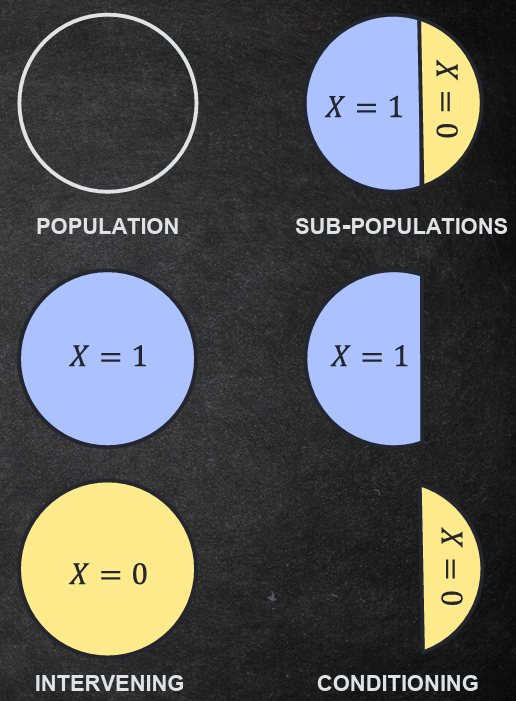
\includegraphics[width=0.3\linewidth]{img/causal_models/interventionVSconditioning.png}
      \caption{Intervention vs Conditioning}
      \label{fig:causal}
\end{figure}

We denote intervention with the \textbf{do-operator} $do(X = x)$. So, if we have
an expression that contains the do-operator, we know that we are intervening
on that variable and we call this expression a \textbf{interventional expression}.
When do do-operator doesn't appear in the expression the expression is called
\textbf{observational expression}.

An \textbf{interventional expression} which can be reduced to an \textbf{observational
      expression} is said to be \textbf{identifiable}. This means that we can
estimate the effect of the intervention from the observational data.

An \textbf{estimand} is said to be:
\begin{itemize}
      \item \textbf{Causal}: whether it does contain the do-operator;
      \item \textbf{Statistical}: it doesn't contain the do-operator.
\end{itemize}

Whenever $do(x)$ appears in the expression after the conditioning bar, it means
that everything in that expression is in the \textbf{post-intervention world}
where intervention $do(x)$ occurs.

\section{Modularity and Adjustment Formula}
We can define a \textbf{causal mechanism} as a mechanism that generates $X_i$ as
the conditional distribution of $X_i$ given its parents (causes) $pa(X_i)$, i.e. $P(X_i | pa(X_i))$.

Also, we want to show that interventions are local. This means that intervening on
a variable $X_i$ only changes the causal mechanism for $X_i$; it does not change
the causal mechanisms that generate any other variables $X_j$.
\begin{definition}[\textbf{Modularity - independent mechanism - invariance of Causal Models}]
      If we intervene on a set of nodes $\mathbf{S}$, setting them to constants,
      then for all $X_i \in \{X_1, \ldots, X_n\}$ we have the following:
      \begin{itemize}
            \item If $X_i \notin \mathbf{S}$ then the causal mechanism that generates
                  $X_i$ ($P(X_i = x | pa(X_i))$) is unchanged by the intervention.
            \item If $X_i \in \mathbf{S}$ then the causal mechanism that generates
                  $X_i$ is replaced by a constant. In other words, $P(X_i | pa(X_i)) = 1$
                  if $x$ is the value that $X_i$ is set to by the intervention
                  $do(X_i = x)$. Otherwise, we have $P(X_i | pa(X_i)) = 0$.
      \end{itemize}
\end{definition}
\begin{note}
      The \textbf{causal graph} for \textbf{interventional (experimental) distributions}
      is simply the same graph that was used for the observational joint distribution,
      but with all of the edges to the intervened node(s) removed.
\end{note}
Using do-expressions and graph surgery, we can begin to untangle the causal
relationships from the purely associative.

Not always modularity is satisfied, for example when we apply $do(X_1 = x)$
and at the same time $P(X_4 = x| X_3)$ changes, in this example modularity wasn't
fulfilled. In reality, this happens when we have hidden factors, so we should
investigate these factors to remove them. See the example on page 20 of the slides.

\begin{note}
      It is worth noting here that we are making a tacit assumption that the
      \textbf{intervention} has no side effects. This means that applying
      intervention this never change values for other variables.
\end{note}

The intervention procedure, which led to the \textbf{Adjustment Formula}, dictates
that $Z$ should coincide with the parents $pa(X)$ of $X$, because it is the
influence of these parents that we neutralize when we fix $X$ by external manipulation
$do(X)$, so we are blocking the association path between $X$ and $Y$ through $Z$,
setting $Z$.

We can therefore write a general Adjustment Formula on a set of variables and
summarize it in a rule:
\begin{definition}[\textbf{Causal effect rule}]
      Given a graph $G$ in which a set of variables $pa(X)$ are designed as the
      parents of a set of variables $X$, the \textbf{causal effect} of $X$ on
      $Y$ can be computed as follows:
      \begin{equation}
            P(Y = y| do(X = x)) = \sum_{u} P(Y | X = x, pa(X) = u)P(pa(X) = u)
      \end{equation}
      where $u$ ranges over all the combinations of values that the variables in
      $pa(X)$ can take, so we are adjusting for $Z$ or controlling for $Z$.
\end{definition}

So we will start from \textbf{causal estimand} $P(Y = y | do(X = x))$ and for the
causal effect rule, we arrive at the \textbf{statistical estimand} which corresponds
to the following expression: $\sum_z P(Y = y|X = x, Z = z) P(Z = z)$ after
the interventions on $X$. This is possible if and only if modularity is satisfied.

If we apply some manipulation to the formula, we can obtain a more convenient
form that is equivalent because we are multiplying and dividing by the same quantity:
\begin{equation}\label{eq:causal_effect_rule}
      P(Y = y| do(X = x)) = \frac{\sum_{u} P(Y = y, X = x, pa(X) = u)P(pa(X) = u)}{P(X = x | pa(X) = u)}
\end{equation}
In the Equation~\ref{eq:causal_effect_rule}, the denominator $P(X = x | pa(X) = u)$
represents the \textbf{propensity score} which displays the role played by the
parents $pa(X)$ of $X$ in determining the result of the intervention $do(X = x)$.

\section{Truncated Factorization and Backdoor Adjustment}
In some circumstances, we can involve multiple interventions at the same time.

The previous consideration also allows us to generalize the Adjustment Formula to
\textbf{multiple interventions}, that is, interventions that fix the values of a
set of variables $\mathbf{S}$ to constants $\mathbf{s}$. We simply write down the
factorization of the preintervention distribution and mark all factors that
correspond to variables in the intervention set $\mathbf{S}$.

\begin{definition}[\textbf{Truncated Factorization (G-formula)}]
      We assume that $P$ and $\mathcal{G}$ satisfy the Markov assumption and modularity.
      Given, a set of intervention nodes $\mathbf{S}$, if $x_i$ is consistent
      with the intervention $\mathbf{S} = \mathbf{s}$, then:
      \begin{equation}
            P(x_1, x_2, \dots, x_n| do(\mathbf{S} = \mathbf{s})) = \prod_{X_i \not \in \mathbf{S}}^{n} P(X_i = x_i | pa(X_i))
      \end{equation}
      otherwise $P(x_1, x_2, \dots, x_n| do(\mathbf{S} = \mathbf{s})) = 0$.
\end{definition}

\begin{note}
      Remember that pre-intervention distribution of a graph $\mathcal{G}$ is
      defined by the Bayesian Network Factorization as follows:
      \begin{equation*}
            P(X_1 = x_1, X_2 = x_2, \dots, X_n = x_n) = \prod_{i = 1}^{n} P(X_i = x_i | pa(X_i))
      \end{equation*}
      While the post-intervention distribution of a graph $\mathcal{G}$ with an
      intervention of $\mathbf{S} = \mathbf{s}$ is defined as followed:
      \begin{equation*}
            P(X_1 = x_1, X_2 = x_2, \dots, X_n = x_n | do(\mathbf{S} = \mathbf{s})) = \prod_{X_i \not \in \mathbf{S}}^{n} P(X_i = x_i | pa(X_i))
      \end{equation*}
      And there is a relationship between them that is defined by:
      \begin{equation*}
            P(X_1 = x_1, X_2 = x_2, \dots, X_n = x_n | do(\mathbf{S} = \mathbf{s})) = \frac{P(X_1 = x_1, X_2 = x_2, \dots, X_n = x_n)}{P(\mathbf{S} = \mathbf{s} | pa(\mathbf{S}))}
      \end{equation*}
      And $P(\mathbf{S} = \mathbf{s} | pa(\mathbf{S}))$ is the \textbf{propensity score}.
\end{note}

Not always in every condition we can use the \textbf{causal effect rule}, in fact,
in the graph represented in the Figure~\ref{fig:unmeasured_parents}, we have
\textbf{unmeasured parents} that impact on $X$ and $Y$, also known as \textbf{latent},
that, though represented in the graph, may be inaccessible for measurement. In
those cases, we can't adjust each value of $pa(X)$ because we can't measure
so we need to find an alternative set of variables to adjust for.
\begin{figure}[!ht]
      \centering
      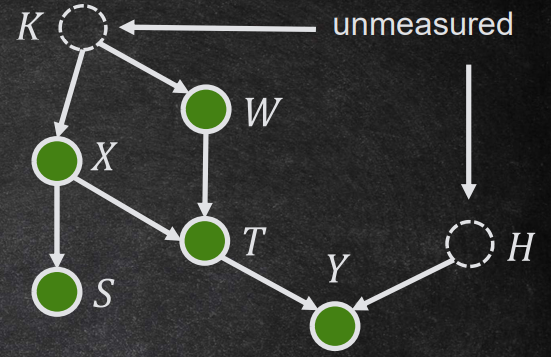
\includegraphics[width=0.4\textwidth]{img/causal_models/unmeasured_parents.png}
      \caption{Unmeasured parents}
      \label{fig:unmeasured_parents}
\end{figure}

\begin{center}
      Under what conditions, is the structure of the causal graph sufficient for
      computing a causal effect from a given data set?
\end{center}

We have decided to represent causal stories with graphs so the solution becomes
a graph theoretical solution.

One of the most important tools we use to determine whether we can compute a
causal effect is a simple test called the \textbf{backdoor criterion}. Using it,
we can determine, for any two variables $X$ and $Y$ in a causal model represented
by a DAG $\mathcal{G}$, which set of variables $\mathbf{S}$ in that model should
be conditioned on when searching for the causal relationship between $X$ and $Y$.

\begin{definition}[\textbf{Backdoor criterion}]
      Given an ordered pair of variables $(X, Y)$ in a DAG $\mathcal{G}$, a set
      of variables $\mathbf{S}$ satisfies the backdoor criterion relative to $(X, Y)$
      if no nodes in $\mathbf{S}$ are descendants of $X$, and $\mathbf{S}$ blocks
      all \textbf{backdoor paths} between $X$ and $Y$ that contain an arrow into $X$.
\end{definition}
\begin{definition}[\textbf{Backdoor paths}]
      A Backdoor path is a path from $X$ to $Y$ when there is an entering arrow
      in $X$.
\end{definition}
\begin{definition}[\textbf{Backdoor adjustment}]
      If a set of variables $\mathbf{S}$ satisfies the backdoor criterion relative
      for $X$ and $Y$, and positivity, then the causal effect of $X$ on $Y$ is
      given by the following new version of the adjusted formula:
      \begin{equation}
            P(Y = y| do(X = x)) = \sum_{\mathbf{s}} P(Y = y| X = x, \mathbf{S} = \mathbf{s})P(\mathbf{S} = \mathbf{s})
      \end{equation}
      just as when we adjust for the parents of $X$ in the Adjustment Formula.
\end{definition}
\begin{note}
      $pa(X)$ satisfied backdoor criterion.
\end{note}

In general, we would like to condition on a set of nodes $\mathbf{S}$ such that we:
\begin{itemize}
      \item Block all the spurious paths between $X$ and $Y$. We want the
            conditioning set $\mathbf{S}$ to block any \textbf{backdoor path} in
            which one end has an arrow into $X$, because such paths may make $X$
            and $Y$ dependent. (confounding effect)
      \item Leave all directed paths from $X$ to $Y$ unchanged. We don't want
            to condition on any nodes that are descendants of $X$.
      \item Create no spurious paths. We should refrain from conditioning on any
            collider that would unblock a new path between $X$ and $Y$.
\end{itemize}
\begin{figure}[!ht]
      \centering
      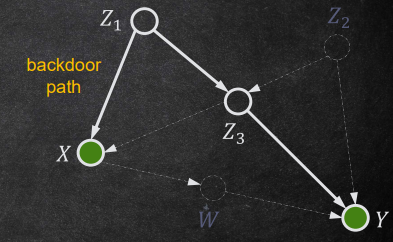
\includegraphics[width=0.4\textwidth]{img/causal_models/backdoor.png}
      \caption{Backdoor paths}
      \label{fig:backdoor}
\end{figure}
\begin{definition}[\textbf{Backdoor Adjustment Formula}]
      Give the modularity assumption, that, $\mathbf{S}$ satisfies the backdoor
      criterion, and positivity, we can identify the causal effect of $X$ on $Y$
      as follows:
      \begin{equation}
            P(Y = y| do(X = x)) = \sum_{\mathbf{s}} P(Y = y| X = x, \mathbf{S} = \mathbf{s})P(\mathbf{S} = \mathbf{s})
      \end{equation}
\end{definition}

We can use the backdoor adjustment formula if, $\mathbf{S}$ d-separates $X$ from
$Y$ in the augmented graph obtained by removing all outgoing edges from $X$.

We would be able to isolate the causal association if $X$ is d-separated from
$Y$ in the augmented graph.
\begin{center}
      \textbf{Isolation of the causal association is identification}
\end{center}

We can also isolate the causal association if $X$ is d-separated from $Y$ in
the augmented graph, conditional on $\mathbf{S}$. This is what the first part of
the backdoor criterion is about and what we've codified in the backdoor adjustment.